En este primer ejercicio hemos implementado el método de verificación de sistemas informáticos consistente en la curva ROC. 
Este sistema de verificación nos permitirá de una manera visual concer las diferentes tasas de error en función del umbral escogido.\par

\section{Datos de entrada}
Las distintas tasas (\textit{scores}) del sistma biométrico las obtenemos mediante ficheros de texto plano, en un ficheros tendremos las tasas de los clientes y en otro las tasas de los impostores.\par


\section{Descripción del trabajo realizado}
Hemos desarrollado un programa en python que lee los ficheros de entrada y que los almacena en una estructura de dattos adecuada para evaluar y consultar el sistema biomédico que estamos evaluando.\par
La estructura básica de esta clase es la que podemos ver en el segmento de código \ref{roc:rocdata}

\begin{lstlisting}[language=python,label=roc:rocdata,caption=EDA con la que gestionar la curva ROC]
class RocData(object):
    def __init__(self, name="", c_score=None, i_score=None):
        self.name = name
        self.c_score = c_score
        self.i_score = i_score
        # Get all possible threasholds and inserts a 0.
        self.thrs = np.unique(
            np.insert(np.concatenate(
                [self.c_score, self.i_score]), 0, 0))
        self.fpr = None
        self.fnr = None
        self.tpr = None
        self.tnr = None

    def solve_ratios(self):
    """ Dado un conjunto de scores obtener los ratios """

    def plot(self, save_path):
    """ Dibujar la curva ROC """

    def aur(self, plot, save_path):
    """ Calcular el área bajo la curva ROC usando 
    el método del trapecio """

    def aur_aprox(self, plot, save_path):
    """ Calcular el área bajo la curva ROC usando 
    un método aproximado """

    def plot_aur(self, aur, save_path):
    """ Dibujar el área bajo la curva ROC """    
    
    def dprime(self, plot):
    """ Obtener el valor D' """

\end{lstlisting}

Además de esto hemos desarrollado el script que lee los ficheros, recoge los argumentos y llama a las disntintas funciones para resolver la curva ROC. 


\section{Resultados}

\subsection{Uso}
Como comentábamos en el apartado anterior el programa que hemos desarrollado es un script de consola con las opciones que podemos ver en la sección de código \ref{roc:help}

\begin{lstlisting}[language=bash,label=roc:help,caption=Uso del script para calcular la curva ROC]
\$ python roc_curve.py --help
usage: roc_curve.py [-h] [-c C] [-i I] [-fp FP] [-fn FN] 
                    [-p] [-a] [-aA] [-d]
                    [-s FILENAME]

Solve the ROC curve

optional arguments:
  -h, --help            show this help message and exit
  -c C, --clients C     Clients filename
  -i I, --impostors I   Impostors filename
  -fp FP                False positive
  -fn FN                False negative
  -p, --plot            Make plot
  -a, --aur             Get area under the ROC curve 
                        using trapezoidal rule
  -aA, --aurAprox       Get area under the ROC curve 
                        using an aproximation
  -d, --dprime          Get dprime
  -s FILE, --save FILE  Path where save ROC curve plot
\end{lstlisting}

\subsubsection{Curva ROC}
Lo primero que podemos realizar es calcular la curva ROC de un sistema.\par
Para esto, leeremos los datos, calcularemos los ratios y a partir de estos ratios dibujar la curva ROC. Damos al usuario la opción de guardar su gráfica. \par
En el segmento de código \ref{roc:roc}, vemos un ejemplo de cómo se lanzaría este script. Del mismo modo en la figura \ref{fig:roc_curve} vemos las curvas ROC de estos dos sistemas biométricos.\par

\begin{lstlisting}[language=bash,label=roc:roc,caption=Calculo de la curva ROC para sistemas biométricos]

$ python roc_curve.py -c ../data/scores/scoresB_clientes.txt 
  -i ../data/scores/scoresB_impostores.txt  -s scoresB
$ python roc_curve.py -c ../data/scores/scoresA_clientes.txt 
  -i ../data/scores/scoresA_impostores.txt  -s scoresA

\end{lstlisting}

\begin{figure}[ht]
    \centering
        \begin{subfigure}[b]{0.5\textwidth}
                \centering
                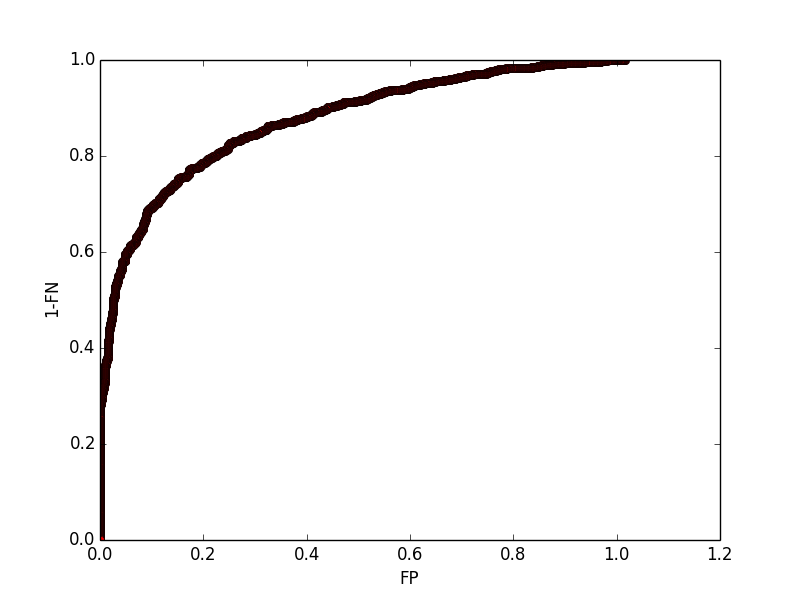
\includegraphics[scale=0.4]{../roc/outputs/scoresA.png}
                \caption{Curva ROC del sistema biométrico A}
                \label{fig:rocA}
        \end{subfigure}%
        \begin{subfigure}[b]{0.5\textwidth}
                \centering
                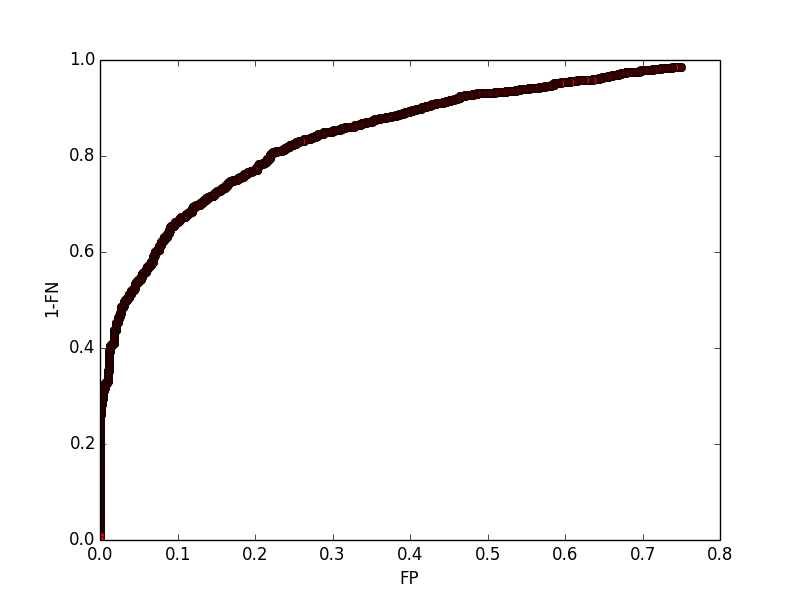
\includegraphics[scale=0.4]{../roc/outputs/scoresB.png}
                \caption{Curva ROC del sistema biométrico b}
                \label{fig:rocB}
        \end{subfigure}
    \caption{Curva ROC para dos sistemas biométricos}\label{fig:roc_curve}
\end{figure}
\newpage
\subsubsection{Obtener el valor FNR o el valor de FPR}
Uno de los datos que nos puede interesar para comparar dos sitemas biométricos o incluso para establecer el valor a partir del cual aceptamos o rechazamos, es que dado el valor del ratio de los falsos positivos obtener el valor del  ratio de los falsos negativos y el umbral para obtener este valor. Análogamente podemos querer el valor de los falsos postivos y el umbral dado un valor de falsos negativos.\par
Podemos ver un ejemplo de la ejecucición en el segmento de código \ref{roc:ratios}.\par

\begin{lstlisting}[language=python,label=roc:ratios,caption=Obtención de ratios y umbrales]

$ python roc_curve.py -c ../data/scores/scoresB_clientes.txt 
-i ../data/scores/scoresB_impostores.txt  -fp 0.6   
Dado el valor de fp: 0.6, el valor 
de fnr es: 0.0458041958042 y el umbral: 0.00434 

$ python roc_curve.py -c ../data/scores/scoresB_clientes.txt 
-i ../data/scores/scoresB_impostores.txt  -fn 0.3 -p
Dado el valor de fn: 0.3, el valor 
de fpr es: 0.129020979021 y el umbral: 0.079034 

\end{lstlisting}

Antes de continuar a la siguiente sección, aclaramos que los valores obtenidos en este apartado se obtienen si existen directamente de los datos y sino se interpolan a partir de la curva ROC.\par

\subsubsection{Obtener el área bajo la curva ROC}

El área bajo la curva ROC es una buena medida para evaluar numéricamente varios sistemas biométricos.\par
Hemos implementado esta medida mediante una aproximación a la integral de la curva y mediante la resolución de la integral mediante el método del trapecio. De los resultados que podemos ver en el segmento de código \ref{roc:aur}, vemos que tanto el área como los tiempos de ejecución varian en función del método empleado.\par
En la figura \ref{fig:aur}, vemos los resultados que hemos obenido.

\begin{lstlisting}[language=bash,label=roc:aur,caption=Calculo del área bajo la curva ROC para sistemas biométricos]
\$ python roc_curve.py -c ../data/scores/scoresB_clientes.txt 
-i ../data/scores/scoresB_impostores.txt  -a       
El área bajo la curva roc es igual a 0.624729082107 
(Coste temporal: 0.000113964080811)

\$ python roc_curve.py -c ../data/scores/scoresB_clientes.txt 
-i ../data/scores/scoresB_impostores.txt  -aA
El área bajo la curva roc es igual a 0.883082526448 
(Coste temporal : 5.70780491829)
\end{lstlisting}

\begin{figure}[ht]
    \centering
        \begin{subfigure}[b]{0.5\textwidth}
                \centering
                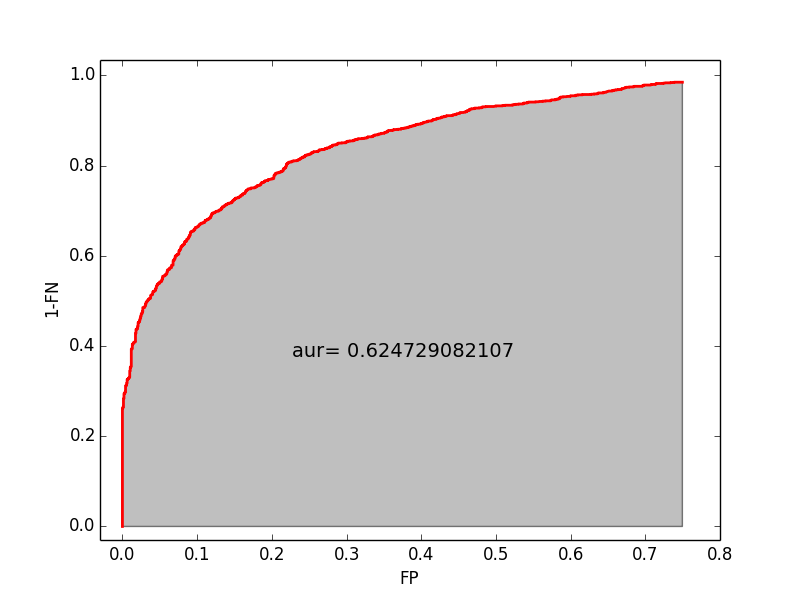
\includegraphics[scale=0.4]{../roc/outputs/aurB_metodo1.png}
                \caption{AUR método aproximado}
                \label{fig:aurAprox}
        \end{subfigure}%
        ~ 
        \begin{subfigure}[b]{0.5\textwidth}
                \centering
                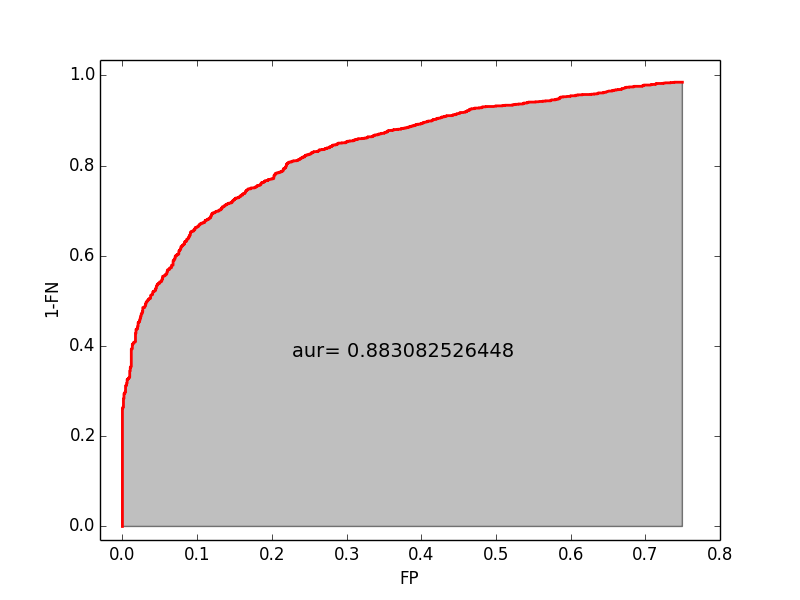
\includegraphics[scale=0.4]{../roc/outputs/aurB_metodo2.png}
                \caption{AUR método del trapecio}
                \label{fig:aurTrap}
        \end{subfigure}
    \caption{AUR}\label{fig:aur}
\end{figure}


\subsubsection{Obtener el factor d'}
Por útlimo calculamos el valor del factor d', que mide la discriminalidad de la técnica empleada. En el segmento de código \ref{roc:dprime} 

\begin{lstlisting}[language=python,label=roc:dprime,caption=Calculo del factor d-prime]
\$ python roc_curve.py -c ../data/scores/scoresB_clientes.txt 
-i ../data/scores/scoresB_impostores.txt  -d -s dprime
El factor dprime es 0.873481856448
\end{lstlisting}
